\documentclass{beamer}
\usepackage{listings}
\lstset{language=C, frame=single, breaklines=true, columns=fullflexible}
\usepackage{hyperref}
\usepackage{subcaption}
\usepackage{url}
\usepackage{tikz}
\usepackage{graphicx}
\usepackage{multicol}
\usepackage{tkz-euclide} % loads  TikZ and tkz-base
%\usetkzobj{all}
\usetikzlibrary{calc,math}
\usetikzlibrary{shapes,arrows.meta,automata, positioning}
\usepackage{float}
\usepackage{amsthm}
\usepackage{mathtools}
\DeclarePairedDelimiter\ceil{\lceil}{\rceil}
\DeclarePairedDelimiter\floor{\lfloor}{\rfloor}
\newcommand\norm[1]{\left\lVert#1\right\rVert}
\renewcommand{\vec}[1]{\mathbf{#1}}
\newcommand{\R}{\mathbb{R}}
\newcommand{\C}{\mathbb{C}}
\newcommand{\comb}[2]{{}^{#1}\mathrm{C}_{#2}}
\providecommand{\brak}[1]{\ensuremath{\left(#1\right)}}
\providecommand{\abs}[1]{\vert#1\vert}
\providecommand{\fourier}{\overset{\mathcal{F}}{ \rightleftharpoons}}
\providecommand{\sbrak}[1]{\ensuremath{{}\left[#1\right]}}
\usepackage[export]{adjustbox}
\usepackage[utf8]{inputenc}
\usepackage{amsmath}
\usepackage[version=4]{mhchem}
\usetheme{Boadilla}
\title{Conditional Probability Voting Algorithm Based on Heterogeneity of Mimic Defense System}
\author{V Rahul}
\institute{IITH}
\date{\today}
\begin{document}
\begin{frame}
    \titlepage
\end{frame}
\begin{frame}{About the paper}
    \begin{block}{Authors}
        \begin{enumerate}[]
            \item Shuai Wei
            \item Huihua Zhang
            \item Wenjian Zhang
            \item Hong Yu
        \end{enumerate}
    \end{block}
    \begin{block}{Institute}
        \begin{enumerate}[]
            \item PLA Strategic Support Force Information Engineering University
            \item Wuxi Xinwu Confidential Technology Service Center
        \end{enumerate}
    \end{block}
    \begin{block}{Date of Publishing}
        \begin{enumerate}[]
            \item October 15, 2020
        \end{enumerate}
    \end{block}
\end{frame}
\begin{frame}{Abstract}
    \begin{block}{}
        \begin{enumerate}
            \item In recent years network attacks have been increasing rapidly, and it is difficult to defend against these attacks, especially attacks at unknown vulnerabilities or backdoors.
            \item As a novel method, Mimic defense architecture has been proposed to solve these cyberspace security problems by using the principle of dynamic heterogeneous redundant variants.
            \item Choosing appropriate variants and voting algorithm according to heterogeneities of these variants become the key issue of designing mimic defense architecture. 
            \item This paper analyzes the system failure probability and scalability of 3 different voting algorithms- MHA, MVA, CPVA, and decide which one is the best.
        \end{enumerate}
    \end{block}
\end{frame}
\begin{frame}{Variants}
    Mimic defense system can be considered a restrict version of N-variant systems, because it adopts the basic idea of running multiple variants of the same program in parallel.
    \begin{block}{}
        \begin{enumerate}
            \item Variants are usually composed of a series of components, such as CPU, operating system, middleware, application, etc.
            \item Each component is composed of several modules. For example, the application can be divided into module 1, module 2,. . ., module M, etc. 
            \item A module is atomic, and its implementations are different from each other. 
            \item Each variant can be represented by a module implementation vector $z^i=({g_1}^i{g_2}^i...{g_N}^i)$, where N is the number of modules contained in a variant and each module may have several implementations. 
        \end{enumerate}
    \end{block}
\end{frame}
\begin{frame}{Variants}
    \begin{figure}[!]
        \centering
        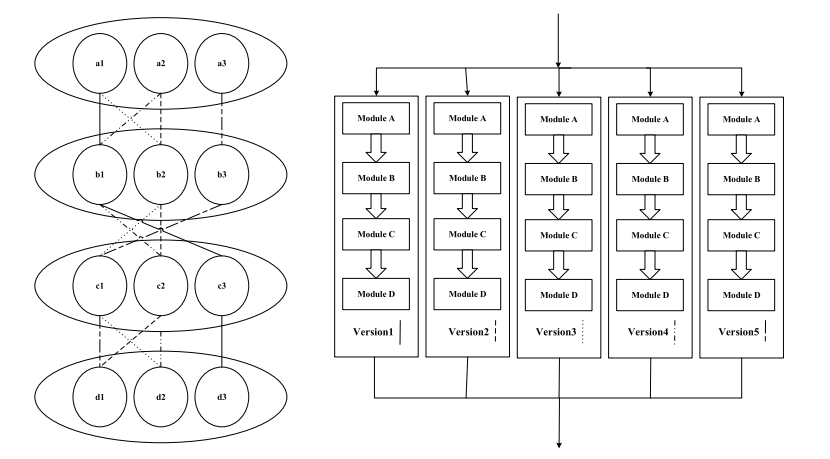
\includegraphics[width = 0.8\columnwidth]{Variant.png}
        \caption{A typical mimic defense instance}
    \end{figure}
\end{frame}
\begin{frame}{Variants}
    The mimic defense system shown in above figure can be described by a matrix as shown below.\\
    \centering
    \begin{pmatrix}
        z^1\\
        z^2\\
        z^3\\
        z^4\\
        z^5\\
    \end{pmatrix}
    =
    \begin{pmatrix}
        a_1 & b_1 & c_3 & d_3\\
        a_2 & b_2 & c_2 & d_1\\
        a_1 & b_2 & c_1 & d_2\\
        a_2 & b_1 & c_2 & d_2\\
        a_3 & b_3 & c_1 & d_1\\
    \end{pmatrix}
\end{frame}
\begin{frame}{Heterogeneous Variants}
    \begin{block}{}
        \begin{enumerate}
            \item Mimic defense system requires the variants to be heterogeneous to each other, not just applications, but also including CPU, OS, middleware and so on.
            \item For a large system which is common in mimic defense system, it is hard to realize totally heterogeneous. 
        \end{enumerate}
    \end{block}
    There are mainly three kinds of algorithms to choose variants: 
    \begin{block}{}
        \begin{enumerate}
            \item maximum heterogeneous algorithm (MHA)
            \item optimal mean distance algorithm (OMDA) 
            \item random seeds scheduling method 
        \end{enumerate}
    \end{block}
\end{frame}
\begin{frame}{Heterogeneous Variants}
    \begin{block}{2-level similarity}
    Suppose there are three variants (1, 2, 3), the 2-level similarities are referred to the similarities for 1\&2,1\&3,2\&3. The sum of similarities is lower, the system is considered to be safer.
    \end{block}
    \begin{block}{}
        \begin{enumerate}
            \item As the number of working variants grows, 2-level similarity become less important. 
            \item Heterogeneity will reach max when there are 3 variants in the mimic system, and the heterogeneity will drop as variants number increase more than 3.
        \end{enumerate}
    \end{block}
\end{frame}
\begin{frame}{Classic Model}
    \begin{figure}[!]
        \centering
        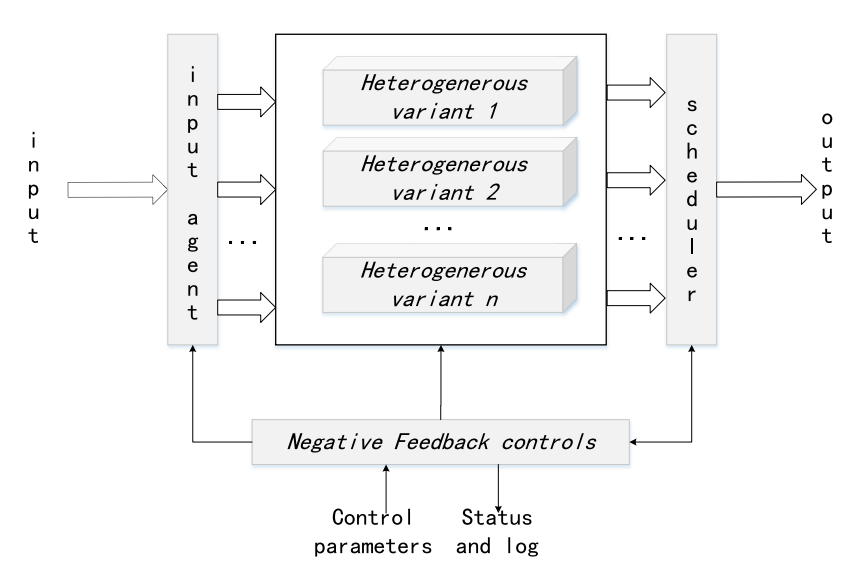
\includegraphics[width = 0.8\columnwidth]{ClassicModel.png}
        \caption{Classic model of mimic defense architecture}
    \end{figure}
\end{frame}
\begin{frame}{Assumptions}
    \begin{block}{}
        \begin{enumerate}
            \item Input agent, Scheduler, and Feedback controller are safe from network attacks.
            \item Each vulnerability/backdoor of the system have the same probability being attacked.
            \item When the high-level vulnerability/backdoor is attacked, the variants who share the vulnerability will generate the same output.
            \item Only one vulnerability / back door can be attacked at a time, and the attacked variant will be cleaned in a short time.
        \end{enumerate}
    \end{block}
    The probability of successfully attacking each module is $\beta_i$ , which should satisfy $\sum_{i}\sum_{\psi_i} \beta_i = 1$, $\psi_i$ is the number of implementations for module i.
\end{frame}
\begin{frame}{Binary Division Vectors}
    \begin{block}{Module diversity  $\psi_i$}
        The implementation number of the module $g_i$, which can be calculated by formula $\lvert \bigcup\limits_{i}{g_k}^i \rvert$. Implementation set is $(a_1a_1a_1a_2a_3)^T$, then union the contents and get the set \{$a_1a_2a_3$\}, which contain 3 elements, so the diversity of module a is 3.
    \end{block}
    \begin{block}{Binary division vector ${\eta_{i}}^k$}
        \begin{enumerate}
            \item In a module, divide the same implementations into one group and other implementations into another group, and use a vector to represent. Assign corresponding values in the vector of the same implementations to 1 and others to 0.
            \item For example, the implementation of $g_{1}$ is ${(a_{1}a_{1}a_{1}a_{2}a_{3})^T}$, then there are 3 binary division vectors for module $g_1$, the binary division vector of $a_2$ is $(00010)^T$, $a_3$ is $(00001)^T$, $a_1$ is $(11100)^T$.
        \end{enumerate}
    \end{block}
\end{frame}
\begin{frame}{Binary Division Vectors}
    \begin{block}{Complement binary division vector \sim ${\eta_{i}}^k$} 
        which is reversing every element in the binary division vector. Based on the binary division vector $(11100)^T$ of module implementation $a_1$, reverse all the elements in it, and its complement vector will be $(00011)^T$.
    \end{block}
    \begin{block}{Isomorphic number of binary division vector ${\lambda_{i}}^k$}
        The number of elements whose value is equal to 1. There are three 1 in the binary division vector of module implementation $a_{1}$, which is $(11100)^T$, then there are three $a_{1}$, and Isomorphic number of $(11100)^T$ is 3.
    \end{block}
\end{frame}
\begin{frame}{Maximum heterogeneous algorithm}
    \begin{block}{}
        \begin{enumerate}
            \item It is based on 2-level similarity.
            \item $system\: failure\: probability = \frac{no.\: of\: similarities}{no.\: of\: vulnerabilities}$.
            \item
            \begin{pmatrix}
                z^1\\
                z^2\\
                z^3\\
                z^4\\
                z^5\\
            \end{pmatrix}
            =
            \begin{pmatrix}
                a_1 & b_1 & c_3 & d_3\\
                a_2 & b_2 & c_2 & d_1\\
                a_1 & b_2 & c_1 & d_2\\
                a_2 & b_1 & c_2 & d_2\\
                a_3 & b_3 & c_1 & d_1\\
            \end{pmatrix}
            \item system failure probability = $\frac{0+1+1+0+1+2+1+1+1+0}{9}=\frac{8}{12}=\frac{3}{4}$
        \end{enumerate}
    \end{block}
\end{frame}
\begin{frame}{Important Property}
    \begin{block}{}
        \begin{enumerate}
            \item If there are T executions in the mimic defense system, there will be atleast 1 implementation whose isomorphic number is not less than $\floor*{\frac{T+1}{2}}$.
            \item In order to reduce the failure probability of mimic defense system, add different implementation of a module or balance the same implementation of a module so that its maximum implementation is less than $\floor*{\frac{T+1}{2}}$.
        \end{enumerate}
    \end{block}
 \end{frame}
\begin{frame}{Majority voting algorithm}
    \begin{block}{}
        \begin{enumerate}
            \item Divide the variants by their results, put variants with the same result into a group $G_k$ . According to the hypothesis only one vulnerability/backdoor is attacked at a time, so there are usually 2 groups, suppose they are $G_1$ and $G_2$.
            \item If $\lvert G_1 \rvert$ $>$ $\lvert G_2 \rvert$, then select the result of G1 as the final output; otherwise, select the result of G2 as the final output.
            \item Clean the variants which have been arbitrated to be abnormal.
        \end{enumerate}
    \end{block}
\end{frame}
\begin{frame}{Majority voting algorithm}
    \begin{block}{}
        \begin{enumerate}
            \item $V_g$ = NULL
            \item for i = 1: N
            \item for k = 1: $\psi_i$
            \item If(${\lambda_i}^k$ \geq\:$\floor*{\frac{T+1}{2}}$)
            \item add i in $V_g$
            \item endfor
            \item endfor
            \item msum = 0
            \item for each index in $U_g$
            \item msum = msum + $\beta_k$
            \item endfor
        \end{enumerate}
    \end{block}
\end{frame}
\begin{frame}{Conditional probability voting algorithm}
    \begin{block}{}
        \begin{enumerate}
            \item  The variants which generated the same results are divided into one group $G_k$ , generally there are only two groups, assumed as $G_1$ and $G_2$.
            \item If there is the same implementation of one module in both $G_1$ and $G2$, the same module implementation in the $G_1$ and $G_2$ need to be removed, then we can get two eliminated sets $G_1^'$ and $G_2^'$, that is $(z^i-\bigcap\limits_{j \subset G_2}^{}z^j)$ and $(z^i-\bigcap\limits_{j \subset G_1}^{}z^j)$.
            \item If there are multiple implementations of one module in $G_1^'$ or $G_2^'$, we use intersection to eliminate different module implementations, we can get two eliminated sets $G_1^''$ and $G_2^''$, that is $ \bigcap\limits_{i \subset G_1}^{}(z^i-\bigcap\limits_{j \subset G_2}^{}z^j)$ and $\bigcap\limits_{i \subset G_2}^{}(z^i-\bigcap\limits_{j \subset G_1}^{}z^j)$.
        \end{enumerate}
    \end{block}
\end{frame}
\begin{frame}{Conditional probability voting algorithm}
    \begin{block}{}
        \begin{enumerate}
            \setcounter{enumi}{3}
            \item Calculation $\beta_{G_1}$ and $\beta_{G_2}$,
            $\beta_{G_1}$ = $\sum_{k}^{} \beta_k$, if k \in $ \bigcap\limits_{i \subset G_1}^{}(z^i-\bigcap\limits_{j \subset G_2}^{}z^j)$, $\beta_{G_2}$ = $\sum_{k}^{} \beta_k$, if k \in $\bigcap\limits_{i \subset G_2}^{}(z^i-\bigcap\limits_{j \subset G_1}^{}z^j)$.
            \item If $\beta_{G_1}$ $>$ $\beta_{G_2}$, the result of $G_2$ shall be used, otherwise, the result of $G_1$ shall be used.
            \item Clean the abnormal variants which have generated wrong result.
        \end{enumerate}
    \end{block}
\end{frame}
\begin{frame}{Conditional probability voting algorithm}
    \begin{block}{}
        \begin{columns}[T] 
            \begin{column}{.34\textwidth}
                \begin{enumerate}
                    \item $G_u$ = NULL
                    \item for i = 1: N
                    \item for k = 1: $\psi_i$
                    \item if(${\lambda_i}^k$ \geq\: $\floor*{\frac{T+1}{2}}$)
                    \item $G_u$ = union($G_u$,${\eta_i}^k$)
                    \item endif
                    \item endfor
                    \item endfor
                    \item csum = 0
                    \item $G_L$ = $G_S$ = NULL
                    \item for each vctorl in $G_u$
                \end{enumerate}
            \end{column}
            \begin{column}{.36\textwidth}
                \begin{enumerate}
                    \setcounter{enumi}{11}
                    \item for i = 1: N
                    \item for k = 1: $\psi_i$
                    \item if(vctorl == ${\eta_i}^k$)
                    \item add i in $G_L$
                    \item else if(\sim$vctorl$==${\eta_i}^k$)
                    \item add i in $G_S$
                    \item endif
                    \item endfor
                    \item endfor
                    \item lsum = ssum = 0
                    \item for each k in $G_L$
                \end{enumerate}
            \end{column}
            \begin{column}{.36\textwidth}
                \begin{enumerate}
                \setcounter{enumi}{22}
                    \item lsum = lsum + $\beta_k$
                    \item endfor
                    \item for each k in $G_S$
                    \item ssum = ssum + $\beta_k$
                    \item endfor
                    \item if $lsum < ssum$
                    \item csum = csum + lsum
                    \item else
                    \item csum = csum + ssum
                    \item endif
                    \item endfor
                \end{enumerate}
            \end{column}
        \end{columns}
    \end{block}
\end{frame}
\begin{frame}{Results for 3-variants experiment}
    \begin{figure}[!]
        \centering
        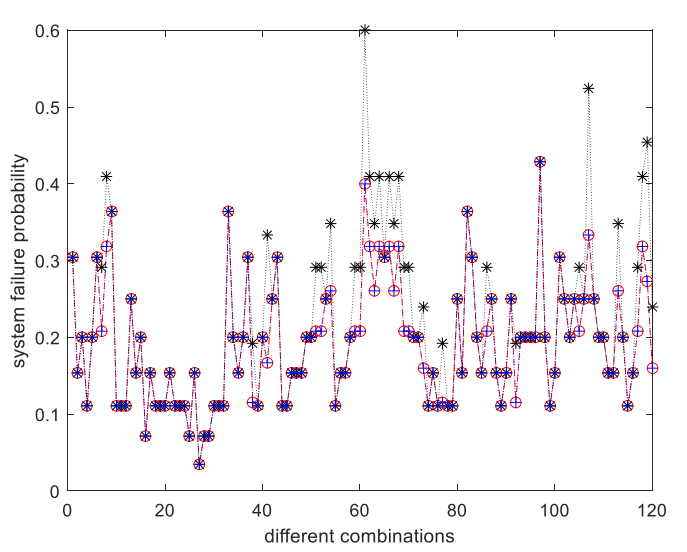
\includegraphics[height = 5cm,width = 0.45\columnwidth]{3variant-1.png}
        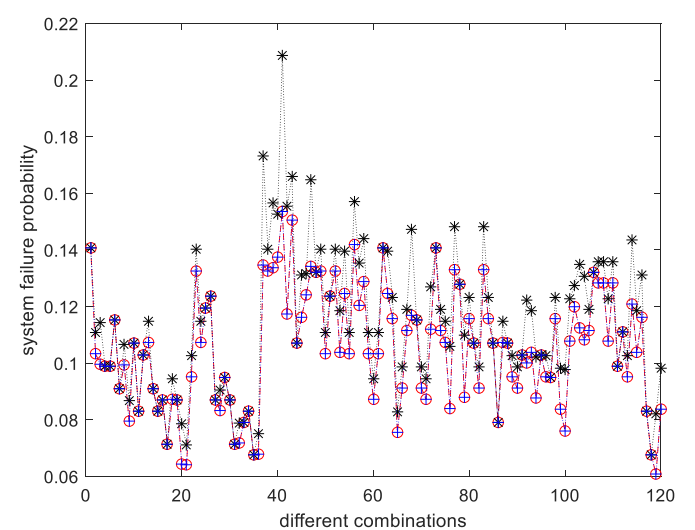
\includegraphics[height = 5cm,width = 0.45\columnwidth]{3variant-2.png}
        \caption{System failure probabilities of MHA, MVA and CPVA when N=10 M=5 and N=100 M=10}
    \end{figure}
\end{frame}
\begin{frame}{Results for 5-variants experiment}
    \begin{figure}[!]
        \centering
        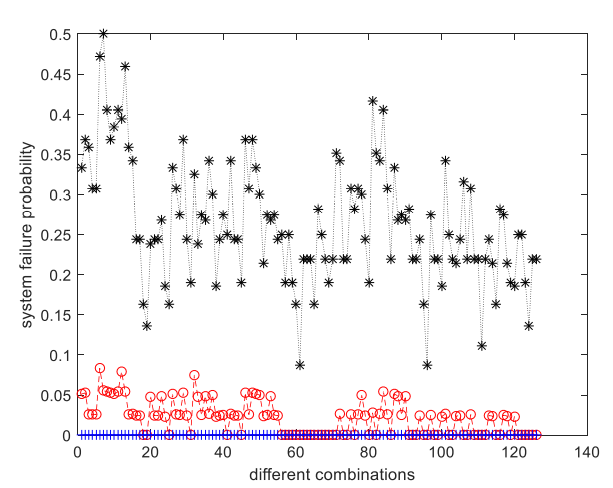
\includegraphics[height = 5cm,width = 0.45\columnwidth]{5variant-1.png}
        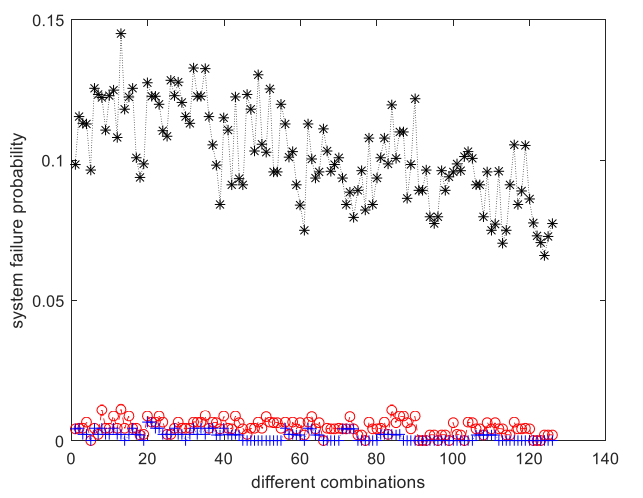
\includegraphics[height = 5cm,width = 0.45\columnwidth]{5variant-2.png}
        \caption{System failure probabilities of MHA, MVA and CPVA when N=10 M=10 and N=100 M=10}
    \end{figure}
\end{frame}
\begin{frame}{Results for scalability experiment}
    \begin{figure}[!]
        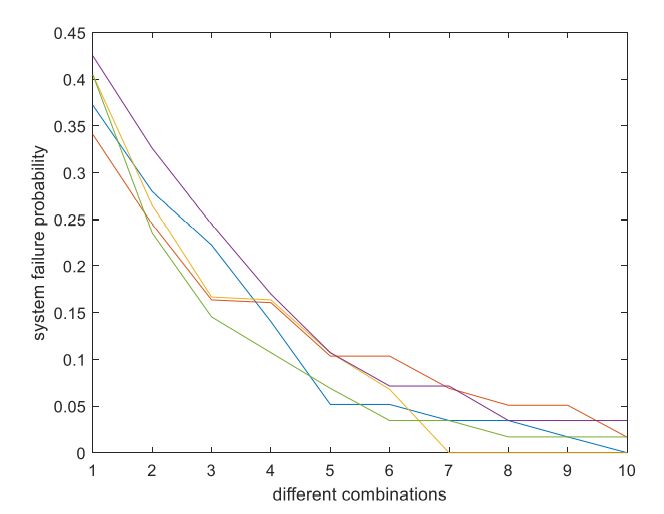
\includegraphics[height = 5cm,width = 0.45\columnwidth]{CPVA.png}
        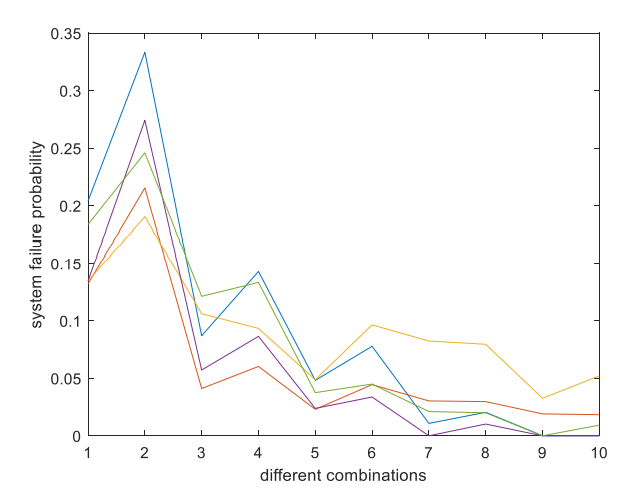
\includegraphics[height = 5cm,width = 0.45\columnwidth]{MVA.png}
        \caption{System failure probabilities of CPVA and MVA with variants increase}
    \end{figure}
\end{frame}
\begin{frame}{Performance analysis}
    \begin{figure}[!]
        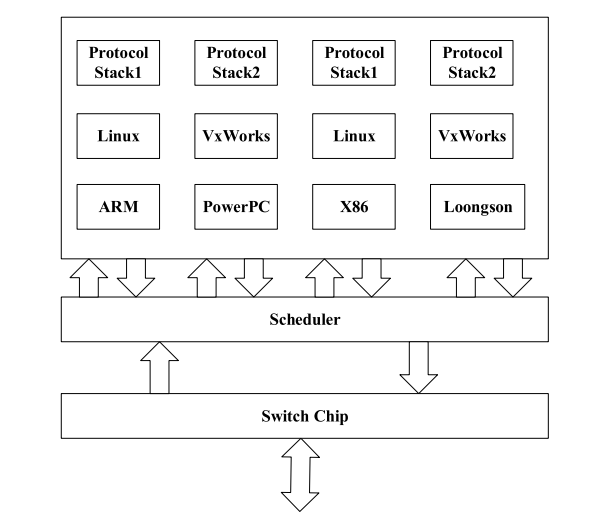
\includegraphics[height = 7cm,width = 0.7\columnwidth]{Ethernet.png}
        \caption{Mimic defense architecture for control panel of ethernet switch.}
    \end{figure}
\end{frame}
\end{document}